%% SW design: klassebeskrivelse UI

\begin{figure}[htbp] \centering
{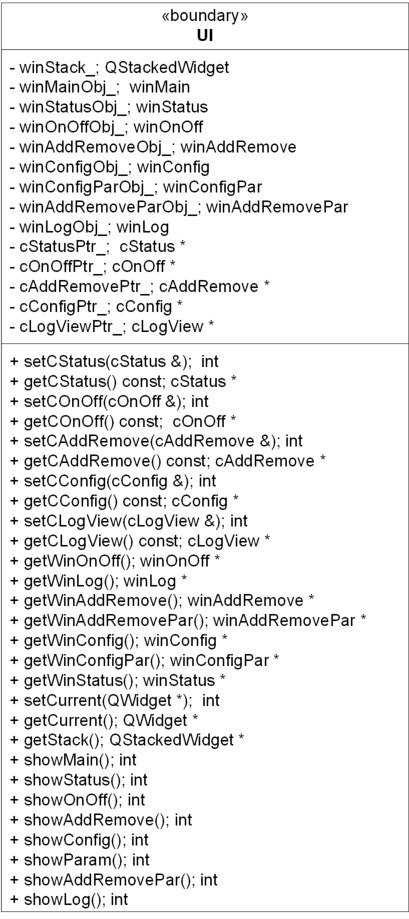
\includegraphics[scale=1.5]{filer/design/Klassediagrammer/sw_UI}}
\caption{Klasse UI}
\label{fig:UI klassediagram}
\end{figure} 

{\centering
\textbf{UI}\par
}
\textbf{Ansvar:} Håndterer alt ved den grafiske brugerflade. \

\textbf{Attributter:}
\begin{itemize}
	\item \verb+QStackedWidget winStack_+ Objekt til at holde alle vinduer i
	\item \verb+winMain winMainObj_+ Hovedmenu vindue
	\item \verb+winStatus winStatusObj_+ Vis status vindue
	\item \verb+winOnOff winOnOffObj_+ Aktiver / Deaktiver vindue
	\item \verb+winAddRemove winAddRemoveObj_+ Tilføj / fjern vindue
	\item \verb+winConfig winConfigObj_+ Konfigurer vindue
	\item \verb+winConfigPar winConfigParObj_+ Konfigurer parametre vindue
	\item \verb+winAddRemovePar winAddRemoveParObj_+ Tilføj Enheds parametre vindue
	\item \verb+winLog winLogObj_+ Vis Log vindue
	\item \verb+cStatus * cStatusPtr_+ Pointer til associeret objekt
	\item \verb+cOnOff * cOnOffPtr_+ Pointer til associeret objekt
	\item \verb+cAddRemove * cAddRemovePtr_+ Pointer til associeret objekt
	\item \verb+cConfig * cConfigPtr_+ Pointer til associeret objekt
	\item \verb+cLogView * cLogViewPtr_+ Pointer til associeret objekt
\end{itemize}

\verb+UI( )+\\
\textbf{Parametre:} Ingen \\
\textbf{Returværdi:} Ingen \\
\textbf{Beskrivelse:} Tilføjer alle \verb+win+-objekterne til stakken \verb+winStack_+. Sætter det aktive vindue til hovedmenuen \verb+winMainObj_+. Indstiller størrelsen på vinduer i stakken til at fylde hele skærmen på Devkit8000, 480x272 og sætter størrelsen på \verb+UI+ til at have samme størrelse. Til sidst opsættes den centrale widget i \verb+QMainWindow+ til stakken \verb+winStack_+.\\

\verb+int setCStatus( cStatus & )+\\
\textbf{Parametre:} Reference til associeret objekt \\
\textbf{Returværdi:} 0 ved succes ellers negativ i overenstemmelse med fejl-listen. \\
\textbf{Beskrivelse:} Sætter medlemspointer til associeret controller.\\

\verb+int setCOnOff( cOnOff & )+\\
\textbf{Parametre:} Reference til associeret objekt \\
\textbf{Returværdi:} 0 ved succes ellers negativ i overenstemmelse med fejl-listen. \\
\textbf{Beskrivelse:} Sætter medlemspointer til associeret controller.\\

\verb+int setCAddRemove( cAddRemove & )+\\
\textbf{Parametre:} Reference til associeret objekt \\
\textbf{Returværdi:} 0 ved succes ellers negativ i overenstemmelse med fejl-listen. \\
\textbf{Beskrivelse:} Sætter medlemspointer til associeret controller.\\

\verb+int setCConfig( cConfig & )+\\
\textbf{Parametre:} Reference til associeret objekt \\
\textbf{Returværdi:} 0 ved succes ellers negativ i overenstemmelse med fejl-listen. \\
\textbf{Beskrivelse:} Sætter medlemspointer til associeret controller.\\

\verb+int setCLogView( cLogView & )+\\
\textbf{Parametre:} Reference til associeret objekt \\
\textbf{Returværdi:} 0 ved succes ellers negativ i overenstemmelse med fejl-listen. \\
\textbf{Beskrivelse:} Sætter medlemspointer til associeret controller.\\

\verb+cStatus * getCStatus( ) const+\\
\textbf{Parametre:} Ingen \\
\textbf{Returværdi:} 0 ved succes ellers negativ i overenstemmelse med fejl-listen. \\
\textbf{Beskrivelse:} Returnerer pointer til associeret objekt.\\

\verb+cOnOff * getCOnOff( ) const+\\
\textbf{Parametre:} Ingen \\
\textbf{Returværdi:} 0 ved succes ellers negativ i overenstemmelse med fejl-listen. \\
\textbf{Beskrivelse:} Returnerer pointer til associeret objekt.\\

\verb+cAddRemove * getCAddRemove( ) const+\\
\textbf{Parametre:} Ingen \\
\textbf{Returværdi:} 0 ved succes ellers negativ i overenstemmelse med fejl-listen. \\
\textbf{Beskrivelse:} Returnerer pointer til associeret objekt.\\

\verb+cConfig * getCConfig( ) const+\\
\textbf{Parametre:} Ingen \\
\textbf{Returværdi:} 0 ved succes ellers negativ i overenstemmelse med fejl-listen. \\
\textbf{Beskrivelse:} Returnerer pointer til associeret objekt.\\

\verb+cLogView * getCLogView( ) const+\\
\textbf{Parametre:} Ingen \\
\textbf{Returværdi:} 0 ved succes ellers negativ i overenstemmelse med fejl-listen. \\
\textbf{Beskrivelse:} Returnerer pointer til associeret objekt.\\

\verb+winOnOff * getWinOnOff( )+\\
\textbf{Parametre:} Ingen \\
\textbf{Returværdi:} 0 ved succes ellers negativ i overenstemmelse med fejl-listen. \\
\textbf{Beskrivelse:} Returnerer pointer til associeret objekt.\\

\verb+winLog * getWinLog( )+\\
\textbf{Parametre:} Ingen \\
\textbf{Returværdi:} 0 ved succes ellers negativ i overenstemmelse med fejl-listen. \\
\textbf{Beskrivelse:} Returnerer pointer til associeret objekt.\\

\verb+winAddRemove * getWinAddRemove( )+\\
\textbf{Parametre:} Ingen \\
\textbf{Returværdi:} 0 ved succes ellers negativ i overenstemmelse med fejl-listen. \\
\textbf{Beskrivelse:} Returnerer pointer til associeret objekt.\\

\verb+winAddRemovePar * getWinAddRemovePar( )+\\
\textbf{Parametre:} Ingen \\
\textbf{Returværdi:} 0 ved succes ellers negativ i overenstemmelse med fejl-listen. \\
\textbf{Beskrivelse:} Returnerer pointer til associeret objekt.\\

\verb+winConfig * getWinConfig( )+\\
\textbf{Parametre:} Ingen \\
\textbf{Returværdi:} 0 ved succes ellers negativ i overenstemmelse med fejl-listen. \\
\textbf{Beskrivelse:} Returnerer pointer til associeret objekt.\\

\verb+winConfigPar * getWinConfigPar( )+\\
\textbf{Parametre:} Ingen \\
\textbf{Returværdi:} 0 ved succes ellers negativ i overenstemmelse med fejl-listen. \\
\textbf{Beskrivelse:} Returnerer pointer til associeret objekt.\\

\verb+winStatus * getWinStatus( )+\\
\textbf{Parametre:} Ingen \\
\textbf{Returværdi:} 0 ved succes ellers negativ i overenstemmelse med fejl-listen. \\
\textbf{Beskrivelse:} Returnerer pointer til associeret objekt.\\

\verb+QStackedWidget * getStack( )+\\
\textbf{Parametre:} Ingen \\
\textbf{Returværdi:} 0 ved succes ellers negativ i overenstemmelse med fejl-listen. \\
\textbf{Beskrivelse:} Returnerer pointer til winStack-objektet.\\

\verb+int showMain( )+\\
\textbf{Parametre:} Ingen \\
\textbf{Returværdi:} 0 ved succes ellers negativ i overenstemmelse med fejl-listen. \\
\textbf{Beskrivelse:} Sætter aktive vindue i \verb+winStack_+-objektet til \verb+winMainObj_+.\\

\verb+int showStatus( )+\\
\textbf{Parametre:} Ingen \\
\textbf{Returværdi:} 0 ved succes ellers negativ i overenstemmelse med fejl-listen. \\
\textbf{Beskrivelse:} Sætter aktive vindue i \verb+winStack_+-objektet til \verb+winStatusObj_+.\\

\verb+int showOnOff( )+\\
\textbf{Parametre:} Ingen \\
\textbf{Returværdi:} 0 ved succes ellers negativ i overenstemmelse med fejl-listen. \\
\textbf{Beskrivelse:} Sætter aktive vindue i \verb+winStack_+-objektet til \verb+winOnOffObj_+.\\

\verb+int showAddRemove( )+\\
\textbf{Parametre:} Ingen \\
\textbf{Returværdi:} 0 ved succes ellers negativ i overenstemmelse med fejl-listen. \\
\textbf{Beskrivelse:} Sætter aktive vindue i \verb+winStack_+-objektet til \verb+winAddRemoveObj_+.\\

\verb+int showConfig( )+\\
\textbf{Parametre:} Ingen \\
\textbf{Returværdi:} 0 ved succes ellers negativ i overenstemmelse med fejl-listen. \\
\textbf{Beskrivelse:} Sætter aktive vindue i \verb+winStack_+-objektet til \verb+winConfigObj_+.\\

\verb+int showParam( )+\\
\textbf{Parametre:} Ingen \\
\textbf{Returværdi:} 0 ved succes ellers negativ i overenstemmelse med fejl-listen. \\
\textbf{Beskrivelse:} Sætter aktive vindue i \verb+winStack_+-objektet til \verb+winConfigParObj_+.\\

\verb+int showAddRemovePar( )+\\
\textbf{Parametre:} Ingen \\
\textbf{Returværdi:} 0 ved succes ellers negativ i overenstemmelse med fejl-listen. \\
\textbf{Beskrivelse:} Sætter aktive vindue i \verb+winStack_+-objektet til \verb+winAddRemoveParObj_+.\\

\verb+int showLog( )+\\
\textbf{Parametre:} Ingen \\
\textbf{Returværdi:} 0 ved succes ellers negativ i overenstemmelse med fejl-listen. \\
\textbf{Beskrivelse:} Sætter aktive vindue i \verb+winStack_+-objektet til \verb+winLogObj_+.\\

